\section{Lab Script}
\setcounter{equation}{0}
\setcounter{figure}{0}

\begin{figure}[h]
    \centering
    
\includegraphics[width=\textwidth]{prototype/UCLlogo.png}
\end{figure}
\bigskip

\begin{center}
\textbf{{\Large Department of Physics \& Astronomy}}

\textbf{{\Large Group Project}}

\textbf{{\Large Course PHAS3441}}

\end{center}
\bigskip

\begin{center}
\noindent\textbf{{\LARGE Cost Effective Demonstration of Wave-Particle Duality on a Table-top}}
\end{center}
\bigskip

\noindent \textbf{Experimental Objectives:}

\begin{enumerate}
\item To understand the principles and conditions for bouncing droplets

\item To determine the driving frequency for differing liquid viscosities

\item To determine the acceleration thresholds for various regimes of droplet motion

\item To observe bouncing, walking and interacting (orbiting, repelling and crystalline lattice structure)

\item To investigate wave-particle duality through various experiments and relate the observed phenomena to theoretical predictions

\item To create a table-top system that can be used by educators for academic purposes
\end{enumerate}
\clearpage
\subsection{Introduction}

In 2005, a team of Physicists showed that silicone oil droplets bouncing on a vibrating tray of the same oil can display wave-particle phenomena. In this project you will be assembling a table-top bouncing oil droplet experiment to demonstrate features of quantum mechanics with basic mechanics such as simple harmonic motion (SHM). This project assumes basic knowledge around Classical Mechanics and Quantum Physics. Recommended knowledge in quantum mechanical phenomena includes: Young’s double slit experiment, quantised energy levels of atomic states, quantum tunnelling into classical forbidden potential and the Pauli Principle.


\subsection{Theory}

The experiment consists of a 4” wide petri dish filled with silicone oil, driven by a loudspeaker situated at the bottom of the petri dish. The driving signal is produced by a Synchronized Function Generator (SFG), which is fed into an amplifier. The SGF produces sinusoidal waves which translate to periodic vibrations of the speaker, providing a mechanical force to accelerate the petri dish vertically. The driving frequency is kept constant, but the amplitude A0 can be varied through adjusting on the SFG. This changes the peak acceleration of the oil bath given by \cite{harris2017visualization}:

\begin{equation}
\gamma =A_0{\omega }^2
\label{equ:vert_acc}
\end{equation}

Where $\omega =2\pi f$ is the angular frequency of the driving force. From \ref{equ:vert_acc} it is suggested that the acceleration is analogous to that of a centripetal acceleration if amplitude is replaced with radius.

It was discovered that specific ranges of peak acceleration will exhibit peculiar, non-classical behaviours. When the experimental acceleration is above a critical acceleration, such as ${\gamma }_B$, a droplet will not coalesce, but bounces indefinitely on the surface of the vibrating bath \cite{brady2014bouncing}. At  higher accelerations above a threshold frequency ${\gamma }_W$, the bouncing state gains a horizontal impulse through interactions with wave-front, which results in a walking state where the droplet moves parallel to the surface by continuously interacting with its own wave. This is analogous to jumping on a trampoline that is placed on a slant surface and having perfectly timed jumps that end up on the next trampoline. This creates a horizontal force even though the driving force only acts vertically. Then, with further increase of acceleration above ${\gamma }_F$, the surface exhibits Faraday instability whereby the surface becomes unstable, causing the droplet to move in an irregular pattern.

\subsection{Apparatus}

The research team of physicists used a SFG, but through the development of smartphones, a simple wave generator application may be installed to act as a function generator. An alternative option would include using a web-based function generator. Using a mobile device will require an amplifier in order to provide enough power for the loudspeaker to excite droplets. In both setups, an LED strip may be fixed around the petri dish to enhance visibility. Although this requires a power source which can be supplied through a USB port. 

The following lists describes the equipment needed for a working setup, as well as extensions to improve the design. Please note that an alternative liquid sample has been proposed: diluted washing up liquid. A similar setup has been carried out before by other physicists, this is shown in Figure \ref {fig:expapparatus}.

\begin{enumerate}
\item  Loudspeaker

\item  Rigid circular wooden plate

\item  Foldback clips (3 - 4")

\item  Banana plugs and crocodile clips

\item  Amplifier

\item  Amplifier power supply cable

\item  4'' petri dish

\item  Wooden apparatus box

\item  Needle

\item  50 cSt silicone oil / washing up liquid  and water

\item  Double-sided tape

\item  Graph paper / black paper

\item  3.5 mm jack to aux cable

\item  Smartphone with function generator app installed or internet access

\item  LED strip

\end{enumerate}

\begin{figure}[h]
    \centering
    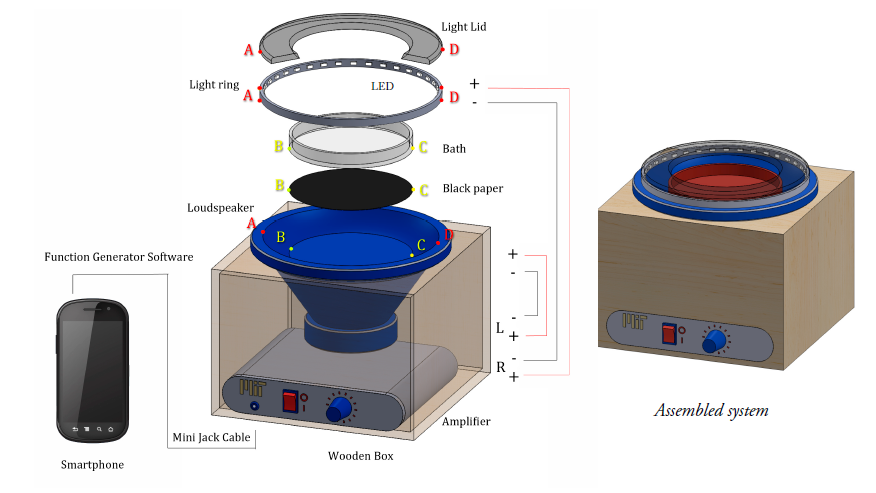
\includegraphics[width=\textwidth]{prototype/Apparatus_Diagram.png}
    \caption{Detailed breakdown of assembled system. This standalone setup uses a smartphone as the function generator \cite{harris2017visualization}.}
    \label{fig:expapparatus}
\end{figure}


\subsection{Assembly Procedure}

\begin{enumerate}

\item \textit{Assembling the wooden apparatus box}: The wooden pieces can be interconnected without any adhesive medium as the finger joints allow the pieces to slot together. Using this, assemble the wooden apparatus box as shown in Figure \ref{fig:WoodenBox}.

\begin{figure}[h]
    \centering
    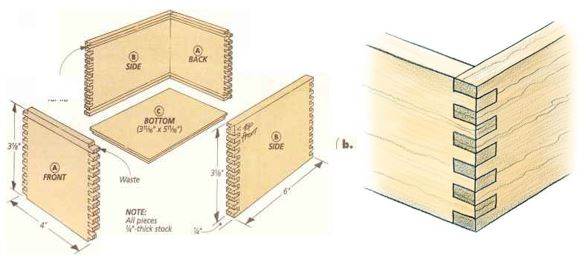
\includegraphics[width=\textwidth]{prototype/WoodenBox.jpg}
    \caption{Assembly of wooden apparatus box that will be used to contain and secure the loudspeaker. (Left) The typical pieces and dimensions of wood \cite{boxdimensions}. (Right)  Secured through slotting the finger joints together \cite{fingerjoints}.}
    \label{fig:WoodenBox}
\end{figure}

\item  \textit{Mounting}: Place the loudspeaker in the wooden apparatus box, ensuring that the connectors are facing an open end to connect cables. To secure the loudspeaker, a variety of methods can be used. Due to the weight of the loudspeaker, it should rest stably in the box, but further securing can be done using hot glue or screws.

\item  \textit{Vibrating Bath}: Secure the circular wooden plate onto the cone of the loudspeaker using foldback clippers. Tape a sheet of graph paper to the base of the 4” petri dish for greater visibility of droplet size and motions. Apply tape along the edge of the petri dish to prevent deterioration of visuals.

\item  \textit{Fill the bath}: Pour silicone oil into the petri dish, creating a fluid layer of approximately 3 – 4 mm depth. Alternatively, create a diluted washing liquid by mixing dish washer with water. Adjust accordingly to a depth that produces consistent droplets.

\item  \textit{Wiring}: Connect the amplifier to the loudspeaker via crocodile clips. Then connect the aux end to the amplifier and insert the 3.5 mm jack end to the mobile device. Test with sample noise/music to ensure that the amplifier and loudspeaker works.

\item  \textit{Configuring}: Start with the lowest amplitude (volume) then configure the app/webpage to output a sinusoidal waveform at a frequency of 50 – 80 Hz. Steadily increase the amplitude to observe vibrations of the oil surface. The system is now ready to operate.

\item  \textit{More Power}: Both the volume control of the mobile device and the amplifier knobs may be adjusted to increase the volume. Due to the frequency range of interest, the bass knob can also be used to further enhance power.

\end{enumerate}


\subsection{Experimental Methods}

\begin{figure}[b]
    \centering
    \begin{subfigure}{0.32\textwidth}
        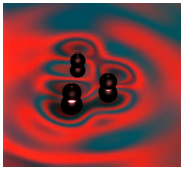
\includegraphics[width=\textwidth]{prototype/BouncingDropletExample.png}
        \caption{Bouncing droplets where $\gamma_W > \gamma > \gamma_B$}
        \label{fig:bouncingdroplets}
    \end{subfigure}
    \begin{subfigure}{0.32\textwidth}
        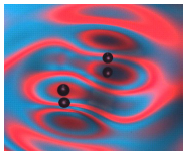
\includegraphics[width=\textwidth]{prototype/WalkingDropletExample.png}
        \caption{Walking droplets where $\gamma_F > \gamma > \gamma_W$}
        \label{fig:walkingdroplets}
    \end{subfigure}
    \begin{subfigure}{0.32\textwidth}
        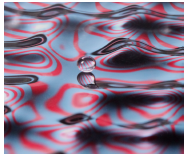
\includegraphics[width=\textwidth]{prototype/IrregularMotionExample.png}
        \caption{Irregular  movements due to Faraday instability where  $\gamma > \gamma_F $}
        \label{fig:faradaydroplets}
    \end{subfigure}
    \caption{Images from \cite{harris2017visualization} of droplets under different regimes.}
    \label{fig:dropletvisualisation}
\end{figure}

\begin{enumerate}

\item \textbf{ }\textit{Bouncing Droplets (Figure \ref{fig:bouncingdroplets})}
\begin{enumerate}
\item  Increase the amplitude on either the mobile device or amplifier, whilst staying below the Faraday threshold (the planar surface of the liquid should remain relatively flat).

\item  Use a needle to create a droplet by dipping it into the bath and then extracting it swiftly. To obtain droplets of bigger size, use a blunter object to create droplets.

\item  Create several droplets and observe their interactions.

\end{enumerate}

\noindent 

\item  \textit{Walking Droplets (Figure \ref{fig:walkingdroplets})}
\begin{enumerate}
\item  Create a bouncing droplet 

\item  Increase the amplitude until the droplet starts to walk. In the case of crossing the Faraday threshold prior to walking, try with other droplet sizes.

\item  Create multiple walkers to observe bound states: orbiting pairs, repelling pairs and crystalline lattices.

\end{enumerate}


\item  \textit{Breaking the Interface (Figure \ref{fig:faradaydroplets}:}

\begin{enumerate} 

\item  Create a few bouncing droplets.

\item  Increase the amplitude even further in order to cross the Faraday threshold. Continue increasing until the surface breaks, creating chaotic waves on the surface.

\item  Observe the droplets undergo irregular motion.

\end{enumerate}


\item\textit{Observations from Diameter -- Acceleration phase diagram \cite{protiere2006particle}}


\begin{itemize}

\item  Diameter and wavelength can be determined using graph paper situated underneath the petri dish

\item  Boundary conditions (BC):
\begin{itemize}
\item  Lowest acceleration BC: bouncing regime at around 1 g (this will be  slightly lower for small drops, due to stored elastic energy)
\item  Highest acceleration BC: Faraday instability (standing waves appearing on whole surface) at around 4.5 g
\item  Quantifying acceleration: fixing treble and bass; model as a linear relationship with the volume knob
\end{itemize}

\item  Regimes for smaller drops ($<$0.8 mm)
\begin{itemize}
\item  Period doubling bouncing at 2.5 g
\item  Period doubling cascade at 3 g
\item  Complicated evolution to walking state
\end{itemize}
\item  Regimes for medium drops (0.8 -- 1.1 mm)
\begin{itemize}
\item  Period doubling
\item  Directly to walking state at around 4 g
\item  Walking state is very near the Faraday instability
\end{itemize}
\item  Regimes for large drops ($>$1.1 mm)
\begin{itemize}
\item  Bouncing indefinitely until Faraday instability
\end{itemize}
\end{itemize}

\item \textit{Bound state and crystalline patterns (extension 1)}

\begin{enumerate}

\item  Set the acceleration to the bouncing regime.
\item  Create two droplets of the same size close to each other.
\item  Increase the acceleration (but remain below period doubling) to observe that bouncers drift towards each other, but stop at a finite distance $d$ where they remain bound.
\item  If the droplets were previously stuck towards each other, the increase in acceleration will cause them to repel one another and stabilise at $d$.
\item  If three droplets were tested, they will form an equilateral triangle of side $d$.
\item  If the droplets were not of the same size, the wave generated by the smaller droplet is weaker, which will cause the bound system to move slowly together.


\end{enumerate}

\item \textit{Orbiting state (extension 2)}



\begin{enumerate}
\item \textbf{ }Create two walkers of the same size, the orbital motion will be symmetric as they are orbiting around their centre of mass.

\item  Test the different stable orbiting radius and verify equation (\ref{equ:orbitingradius})\cite{protiere2006particle}:
\begin{equation}
    {d_n}^{orb}=\left(n-\varepsilon \right){\lambda }_F
    \label{equ:orbitingradius}
\end{equation}

\item  Since the oscillating frequency is half of the driving frequency, droplets can be either in-phase or out of phase.

\item  Decrease the acceleration into the bouncing regime and then increasing back to the walking regime allows the phase to be altered.

\item  By using the same droplets, either a mutual capture or a repulsive collision can be observed.

\item  Droplets of different diameters can also form an orbiting system, with the centre of rotation shifted due to the different velocities of the droplets.
\end{enumerate}

\end{enumerate}
